\let\negmedspace\undefined
\let\negthickspace\undefined
\documentclass[article]{IEEEtran}
\usepackage[a5paper, margin=10mm, onecolumn]{geometry}
\usepackage{tfrupee}

\setlength{\headheight}{1cm}
\setlength{\headsep}{0mm}

\usepackage{gvv-book}
\usepackage{gvv}
\usepackage{cite}
\usepackage{amsmath,amssymb,amsfonts,amsthm}
\usepackage{algorithmic}
\usepackage{graphicx}
\usepackage{textcomp}
\usepackage{xcolor}
\usepackage{txfonts}
\usepackage{listings}
\usepackage{enumitem}
\usepackage{mathtools}
\usepackage{gensymb}
\usepackage{comment}
\usepackage[breaklinks=true]{hyperref}
\usepackage{tkz-euclide} 
\usepackage{listings}                                       
\def\inputGnumericTable{}                                 
\usepackage[latin1]{inputenc}                                
\usepackage{color}                                            
\usepackage{array}                                            
\usepackage{longtable}                                       
\usepackage{calc}                                             
\usepackage{multirow}                                         
\usepackage{hhline}                                           
\usepackage{ifthen}                                           
\usepackage{lscape}

\renewcommand{\thefigure}{\theenumi}
\renewcommand{\thetable}{\theenumi}
\setlength{\intextsep}{10pt}

\numberwithin{figure}{enumi}
\renewcommand{\thetable}{\theenumi}
\begin{document}
\bibliographystyle{IEEEtran}
\title{NCERT-11.16.3.8.2}
\author{EE24BTECH11035 - KOTHAPALLI AKHIL}
{\let\newpage\relax\maketitle}
\noindent\textbf{Question: }  Three coins are tossed once. Find the probability of getting 2 Heads?\\
\solution\\
Textual Method, \\
The Possibilities when 3 coins tossed  are, 
\begin{align}
\left\{\{H,H,H\}, \{H,T,T\}, \{T,H,T\}, \{T,T,H\}, \{T,T,T\}, \{T,H,H\}, \{H,T,H\}, \{H,H,T\}\right\}
\end{align}
The Number of Possible outcomes which have 2 Heads is 4\\
Therefore, Required probability is
\begin{align}
    P=\frac{4}{8}\\
    P=\frac{1}{2}
\end{align}
Computational method,\\
\textbf{Computational Solution:}\\

\section*{Computation of Probabilities for Tossing Three Coins}

To compute the probability of obtaining specific outcomes when tossing three coins, we rely on two key concepts: the **Probability Mass Function (PMF)** and the **Cumulative Distribution Function (CDF)**.

\subsection*{Definitions}
\subsubsection*{Probability Mass Function (PMF)}
The PMF represents the probability of each individual outcome in the sample space $ S $. For three coin tosses:
\begin{align}
S = \{HHH, HHT, HTH, HTT, THH, THT, TTH, TTT\},
\end{align}
the PMF is given as:
\begin{align}
P(X = x) =
\begin{cases}
\frac{1}{8}, & x \in S, \\
0, & x \notin S.
\end{cases}
\end{align}

\subsubsection*{Cumulative Distribution Function (CDF)}
The CDF represents the cumulative probability of outcomes up to a given number of heads $ x $, defined as:
\begin{align}
F(x) = P(X \leq x) = \sum_{k=0}^{x} P(X = k).
\end{align}
For three coin tosses, where $ X $ is the number of heads:
\begin{align}
F(x) =
\begin{cases}
0, & x < 0, \\
\frac{1}{8}, & x = 0, \\
\frac{4}{8}, & x = 1, \\
\frac{7}{8}, & x = 2, \\
1, & x \geq 3.
\end{cases}
\end{align}

\subsection*{Simulation Process}
We simulate the tossing of three coins using the following steps:
\begin{enumerate}
    \item Each coin produces outcomes in the set:
    \begin{align}
    \{H, T\}.
    \end{align}
    \item For each simulated toss, a random outcome is generated for three coins.
    \item The number of occurrences of each outcome is tracked over $ N $ trials, where $ N $ is the total number of simulations.
    \item Both the PMF and CDF are computed:
    \begin{itemize}
        \item **PMF**: The frequency of each outcome (number of heads) is divided by the total trials to compute the probability of each case.
        \item **CDF**: The cumulative probabilities are calculated as the running total of the PMF values.
    \end{itemize}
\end{enumerate}

\subsection*{Calculation of Probabilities}
\subsubsection*{Probability of Each Outcome (PMF)}
The probability of getting exactly $ i $ heads ($ i \in \{0, 1, 2, 3\} $) is computed as:
\begin{align}
P(i) = \frac{\text{Number of trials resulting in } i \text{ heads}}{N}.
\end{align}

\subsubsection*{Cumulative Probability (CDF)}
The cumulative probability of getting up to $ i $ heads is:
\begin{align}
F(i) = \sum_{k=0}^{i} P(k).
\end{align}

\subsubsection*{Probability of Getting At Least 2 Heads}
The probability of getting at least 2 heads is:
\begin{align}
P(X \geq 2) = 1 - P(X < 2) = 1 - F(1).
\end{align}
Given the computed CDF values:
\begin{align}
P(X \geq 2) = 1 - \frac{4}{8} = \frac{4}{8} = \frac{1}{2}.
\end{align}

\subsection*{Output Representation}
The computed probabilities are represented in two forms:
\begin{itemize}
    \item **PMF**: The probabilities of getting $ \{0, 1, 2, 3\} $ heads.
    \item **CDF**: The cumulative probabilities up to each number of heads, $ \{0, 1, 2, 3\} $, showing the cumulative likelihood of outcomes.
\end{itemize}
    \begin{figure}[h!]
        \centering
        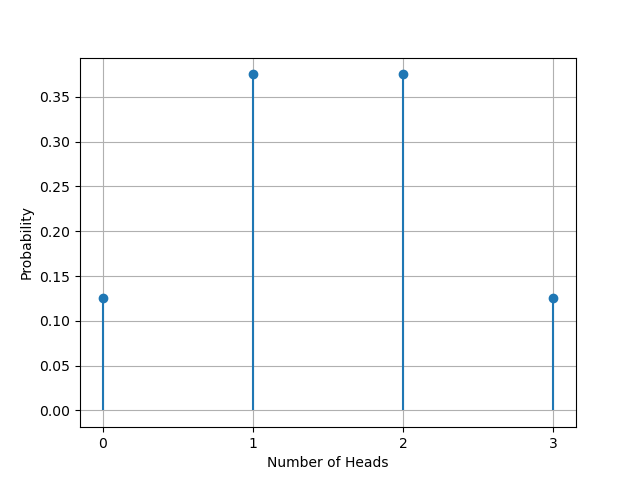
\includegraphics[width=\columnwidth]{figs/fig2.png}
        \caption{Solution of the probability distribution for three coin tosses}
        \label{stemplot2}
    \end{figure}


\end{document}
